\documentclass[12pt]{beamer}
\usetheme{CambridgeUS}
\usepackage[utf8]{inputenc}
\usepackage[spanish]{babel}
\usepackage{amsmath}
\usepackage{multirow, array}
\usepackage{amsfonts}
\usepackage{amssymb}
\usepackage{graphicx}
\usepackage{ragged2e}
\setbeamertemplate{navigation symbols}{} 
\author[Kevin - Alejandro x2]{Kevin García 1533173 \newline Alejandro Vargas 1525953 \newline Alejandro Soto 1532457}
\title[Diseños factoriales fraccionados]{Diseños factoriales fraccionados}

%\setbeamercovered{transparent} 
%\setbeamertemplate{navigation symbols}{} 
%\logo{} 
%\institute{} 
%\date{} 
%\subject{} 
\begin{document}
\justifying
\begin{frame}[plain]
\maketitle
\end{frame}


\begin{frame}
\frametitle{Introducción}
Los diseños factoriales surgen ante la necesidad de estudiar conjuntamente varios factores obedeciendo a la posibilidad de que el efecto de un factor cambie según los niveles de otros factores, esto es, que los factores interactúen. Estos diseños también se usan cuando se quiere
optimizar la respuesta o variable dependiente, es decir, se quiere encontrar la combinación de niveles de los factores que producen un valor óptimo de la variable dependiente.
~\\Si se investiga un factor por separado, el resultado puede ser diferente al estudio conjunto y es mucho más difícil describir el comportamiento general del proceso o encontrar el óptimo.
\end{frame}

\begin{frame}
\frametitle{Diseño Factorial}
~\\Un diseño factorial es un tipo de experimento cuyo diseño permite estudiar los efectos que varios factores pueden tener en una respuesta. Al realizar un experimento, variar los niveles de todos los factores al mismo tiempo en lugar de uno a la vez, permite estudiar las interacciones entre los factores.

\end{frame}

\begin{frame}
\frametitle{Diseño Factorial}
~\\Suponga que tenemos dos factores, $A$ con a niveles y $B$ con b niveles. Las observaciones de un experimento factorial pueden describirse con un modelo. Hay varias formas de escribir el modelo de un experimento factorial. La forma más utilizada es el modelo de los efectos:
\begin{center}
$y_{ijk}=\mu+\tau_i+\beta_j+(\tau\beta)_{ij}+\varepsilon_{ijk} \;\;\; \left \{\begin{array}{c} i=1,2,...,a \\ j=1,2,...,b \\ k=1,2,...,n \end{array}\right. $
\end{center}
\end{frame}


\begin{frame}
\frametitle{Diseño Factorial}

~\\Donde $\mu$ es el efecto promedio global, $\tau_i$ es el efecto del nivel i-ésimo del factor $A$ de los renglones, $\beta_j$ es el efecto del nivel j-ésimo del factor $B$ de las columnas, $(\tau\beta)_{ij}$ es el efecto de la interacción entre $\tau_i$ y $\beta_j$, y $\varepsilon_{ijk}$ es un componente del error aleatorio. Puesto que hay n replicas del experimento, hay $abn$ observaciones en total.

\end{frame}

\begin{frame}
\frametitle{Diseño Factorial}
~\\El efecto de un factor se define como el cambio en la respuesta producido por un cambio en el nivel del factor, a este efecto se le conoce como efecto principal porque se refiere a los factores de interés primario en el experimento. Entonces si tenemos dos factores A y B, como en la siguiente tabla:
~\\
% Table generated by Excel2LaTeX from sheet 'Hoja1'
\begin{table}[htbp]
  \centering
  \caption{}
    \begin{tabular}{|c|c|c|}
\cline{2-3}    \multicolumn{1}{c|}{} & \multicolumn{2}{c|}{\textbf{Factor A}} \\
    \hline
    \textbf{Factor B} & \textbf{bajo } & \textbf{alto} \\
    \hline
    \textbf{bajo} & a     & b  \\
    \hline
    \textbf{alto} & c     & d  \\
    \hline
    \end{tabular}%
  \label{tab:addlabel}%
\end{table}%
\end{frame}

\begin{frame}
\frametitle{Diseño Factorial}
~\\El efecto principal del factor A es la diferencia entre la respuesta promedio con el nivel alto de A y la respuesta promedio con el nivel bajo de A. Esto es:
$$A=\frac{b+d}{2}-\frac{a+c}{2}$$
~\\Análogamente, el efecto principal del factor B es:
$$B=\frac{c+d}{2}-\frac{a+b}{2}$$  
\end{frame}

\begin{frame}
\frametitle{Diseño Factorial}
~\\Si existe interacción entre los factores A y B, el efecto de la interacción se define como la diferencia promedio de los dos efectos del factor A, es decir:
$$AB=\frac{(d-c)-(b-a)}{2}$$
~\\En el diseño factorial de dos factores, ambos factores, $A$ y $B$ son de igual interés, por lo que se prueban las hipótesis acerca de la igualdad de los efectos de los tratamientos de cada factor. Para el factor $A$:
\begin{center}
~\\$H_0:\tau_1=\tau_2=\cdots=\tau_a=0$
~\\$H_1:$Al menos una $\tau_i\neq 0$
\end{center}
\end{frame}

\begin{frame}
\frametitle{Diseño Factorial}
~\\Para el factor $B$:
\begin{center}
~\\$H_0:\beta_1=\beta_2=\cdots=\beta_b=0$
~\\$H_1:$Al menos una $\beta_j\neq 0$
\end{center}
~\\También existe interés en determinar si los tratamientos de los factores $A$ y $B$ interactúan. Por lo tanto, también querría probarse
\begin{center}
~\\$H_0:(\tau\beta)_{ij}=0$ para todas las $i,j$
~\\$H_1:$Al menos una $(\tau\beta)_{ij}\neq 0$
\end{center}
\end{frame}

\begin{frame}
\frametitle{Diseño Factorial}
~\\Todas las hipótesis anteriores se pueden probar realizando el análisis de varianza de dos factores como sigue:

\begin{table}[htbp]
  \centering
  \caption{ANOVA}
\resizebox{12cm}{!} {
\begin{tabular}{|c|c|c|c|c|}
\hline 
Fuente de Variación & Grados de Libertad & Suma de Cuadrados & Cuadrados Medios & F \\ 
\hline 
$A$ & a-1 & $SC_A$ & $CM_A=\frac{SC_A}{a-1}$ & $F=\frac{CM_{A}}{CM_{error}}$ \\ 
$B$ & b-1 & $SC_B$ & $CM_B=\frac{SC_B}{b-1}$ & $F=\frac{CM_{B}}{CM_{error}}$ \\
$AB$ &(a-1)(b-1) & $SC_{AB}$ & $CM_{AB}=\frac{SC_{AB}}{(a-1)(b-1)}$ & $F=\frac{CM_{AB}}{CM_{error}}$ \\
Error & ab(n-1) & $SC_{error}$ & $CM_{error}=\frac{SC_{error}}{ab(n-1)}$ &   \\ 
Total & abn-1 & $SC_{total}$ &  &   \\ 
\hline 
\end{tabular} 
}
\label{tab:addlabel}%
\end{table}%
\end{frame}

\begin{frame}
\frametitle{Diseño Factorial}
~\\Donde la suma de cuadrados total es:
$$SC_{total}=\sum\limits_{i=1}^a \sum\limits_{j=1}^b \sum\limits_{k=1}^n y^2_{ijk}-\frac{y^2_{\ldots}}{abn}$$

~\\La suma de cuadrados de los efectos principales son:
\begin{center}
$SC_A=\frac{1}{bn}\sum\limits_{i=1}^a y^2_{i..} - \frac{y^2_{\ldots}}{abn}\;\;$ y $\;\;SC_B=\frac{1}{an}\sum\limits_{j=1}^b y^2_{.j.} - \frac{y^2_{\ldots}}{abn}$
\end{center}

\end{frame}

\begin{frame}
\frametitle{Diseño Factorial}
~\\La suma de cuadrados de la interacción es:
$$SC_{AB}=\frac{1}{n}\sum\limits_{i=1}^a\sum\limits_{j=1}^b y^2_{ij.}-\frac{y^2_{\ldots}}{abn}-SC_{A}-SC_{B}$$

~\\Y, la suma de cuadrados del error se encuentra como:
$$SC_{error}=SC_{total}-\frac{1}{n}\sum\limits_{i=1}^a\sum\limits_{j=1}^b y^2_{ij.}-\frac{y^2_{\ldots}}{abn}$$
\end{frame}

\begin{frame}
\frametitle{Diseño Factorial $2^{k}$}
~\\Existen varios casos especiales del diseño factorial general, los cuales son muy importantes debido a su uso generalizado en el trabajo de investigación. El más importante de estos casos especiales es el diseño de k factores, donde cada factor cuenta con sólo dos niveles. Estos niveles pueden ser tanto cuantitativos como cualitativos. Una réplica completa de este diseño requiere $2 x 2 x\cdots x 2 =2^k$ observaciones y se le llama diseño factorial $2^k$.
\end{frame}

\begin{frame}
\frametitle{Diseño Factorial $ 2^{k} $}
~\\El diseño $2^k$ es de particular utilidad en las etapas iniciales del trabajo experimental, cuando probablemente se estén investigando muchos factores. Este diseño proporciona el menor número de corridas con las que pueden estudiarse k factores en un diseño factorial completo.

~\\El modelo estadístico para un diseño $2^k$ incluiría k efectos principales, $\binom{k}{2}$ interacciones de dos factores, $\binom{k}{3}$ interacciones de tres factores,..., y una interacción de k factores. Es decir, para un diseño $2^k$ el modelo completo contendría $2^k-1$ efectos.
\end{frame}

\begin{frame}
\frametitle{Diseño Factorial $ 2^{k} $}

~\\El enfoque general para el análisis estadístico del diseño $2^k$ se resume en la siguiente tabla
\begin{table}[htbp]
  \centering
  \caption{Enfoque del diseño  $ 2^{k} $}
  \resizebox{0.7\textwidth}{!} {
\begin{tabular}{l}
\hline 
1. Estimar los efectos de los factores\\
2. Formar el modelo inicial\\
3. Realizar las pruebas estadísticas\\
4. Refinar el modelo\\
5. Analizar los residuales\\
6. Interpretar los resultados\\
\hline 
\end{tabular}
}
\label{tab:addlabel}%
\end{table}%
\end{frame}

\begin{frame}
\frametitle{Diseño Factorial $ 2^{k} $}
~\\En este diseño, la tabla estándar se construye empezando con el primer factor con el signo(-) y alterna signos (-) y (+). El segundo factor cambia de signo cada dos observaciones ($2^1$), el tercer factor cada cuatro ($2^2$) y el factor k-ésimo cada $2^{k-1}$ observaciones. las interacciones de los factores tienen los signos que se obtienen de multiplicar los signos de los factores implicados. Por ejemplo, en el diseño $2^3$ la tabla estándar con las interacciones es:
\end{frame}

\begin{frame}
\frametitle{Diseño Factorial $ 2^{k} $}
\begin{table}[H]
  \centering
  \caption{Matriz de Diseño}
  \resizebox{0.7\textwidth}{!}{
    \begin{tabular}{cccccccc}
    \hline
    \textbf{A} & \textbf{B} & \textbf{C} & \textbf{AB} & \textbf{AC} & \textbf{BC} & \textbf{ABC} & \textbf{Respuesta y} \\
    \hline
    -     & -     & -     & +     & +     & +     & -     & $y_{111}=(1)$ \\
    +     & -     & -     & -     & -     & +     & +     & $y_{211}=a$ \\
    -     & +     & -     & -     & +     & -     & +     & $y_{121}=b$ \\
    +     & +     & -     & +     & -     & -     & -     & $y_{221}=ab$ \\
    -     & -     & +     & +     & -     & -     & +     & $y_{112}=c$ \\
    +     & -     & +     & -     & +     & -     & -     & $y_{212}=ac$ \\
    -     & +     & +     & -     & -     & +     & -     & $y_{122}=bc$ \\
    +     & +     & +     & +     & +     & +     & +     & $y_{222}=abc$ \\
    \hline
    \end{tabular}%
    }
  \label{tab:addlabel}%
\end{table}%
\end{frame}

\begin{frame}
\frametitle{Diseño Factorial $ 2^{k} $}
~\\En la tabla se logra apreciar que el nivel alto de cualquiera de los factores en una combinación de tratamientos se denota por la letra minúscula correspondiente y que el nivel bajo de un factor en una combinación de tratamientos se denota por la ausencia de la letra respectiva. Por lo tanto, para un diseño $2^2$ a representa la combinación de tratamientos con A en el nivel alto y B en el nivel bajo, b representa A en el nivel bajo y B en el nivel alto, y ab representa ambos factores en el nivel alto. Por convención, se usa (1) para denotar que ambos factores están en el nivel bajo. Esta notación se utiliza en todos los diseños $2^k$.
\end{frame}

\begin{frame}
\frametitle{Diseño Factorial $ 2^{k} $}
~\\Para estimar un efecto o calcular la suma de cuadrados de un efecto, primero debe determinarse el contraste asociado con ese efecto. En general, el contraste del efecto $AB\cdots K$ se determina expandiendo el miembro derecho de
$$Contraste_{AB\cdots K}=(a\pm 1)(b\pm 1)\cdots(k\pm 1)$$
~\\Una vez se han calculado los contrastes de los efectos, pueden estimarse los efectos y calcular las sumas de cuadrados de acuerdo con
$$AB\cdots K=\frac{2}{n2^k}(Contraste_{AB\cdots K})$$
$$SS_{AB\cdots K}=\frac{1}{n2^k}(Contraste_{AB\cdots K})^2$$

\end{frame}

\begin{frame}
\frametitle{Diseño Factorial $ 2^{k} $}
~\\Entonces el análisis de varianza de un diseño $2^k$ es
\begin{table}[H]
  \centering
  \caption{Análisis de varianza diseño $2^k$}
  \resizebox{0.6\textwidth}{!}{
    \begin{tabular}{ccc}
    \hline
    \textbf{Fuente de variación} & \textbf{Suma de cuadrados} & \textbf{Grados de libertad} \\
    \hline
   A & $SS_A$ & 1 \\
   B & $SS_B$ & 1 \\
   \vdots & \vdots & \vdots \\
   K & $SS_K$ & 1 \\
   AB & $SS_{AB}$ & 1 \\
   AC & $SS_{AC}$ & 1 \\
   \vdots & \vdots & \vdots \\
   JK & $SS_{JK}$ & 1 \\
   ABC & $SS_{ABC}$ & 1\\
   ABD & $SS_{ABD}$ & 1\\
   \vdots & \vdots & \vdots\\
   IJK & $SS_{IJK}$ & 1\\
   \vdots & \vdots & \vdots \\
   $ABC\cdots K$ & $SS_{ABC\cdots K}$ & 1\\
   Error & $SS_{E}$ & $2^k(n-1)$ \\
   Total & $SS_{T}$ & $n2^k-1$ \\
    \hline
    \end{tabular}%
    }
  \label{tab:addlabel}%
\end{table}%
\end{frame}

\begin{frame}
\frametitle{Diseños Factoriales Fraccionados}
~\\En un diseño factorial conforme el número de factores del experimento crece, el número de casillas o condiciones experimentales (y por lo tanto el número de lecturas o pruebas necesarias), crece exponencialmente, también crece el número de efectos a evaluar (interacciones principalmente) y el número de efectos y casillas varía con el número de factores en una relación como se muestra en la tabla siguiente para un experimento factorial $2^k$.
\end{frame}

\begin{frame}
\frametitle{Diseño Factorial Fraccionado}
% Table generated by Excel2LaTeX from sheet 'Hoja1'
\begin{table}[htbp]
  \centering
  \caption{No de factores del experimento}
  \resizebox{0.8\textwidth}{!}{
    \begin{tabular}{|c|c|c|c|c|c|c|c|c|c|}
    \hline
    \multicolumn{1}{|c|}{\multirow{2}[4]{*}{\textbf{No. De \newline{} factores}}} & \multicolumn{1}{c|}{\multirow{2}[4]{*}{\textbf{No. De \newline{} casillas}}} & \multicolumn{1}{c|}{\multirow{2}[4]{*}{\textbf{Efectos \newline{} principales}}} & \multicolumn{7}{c|}{\textbf{Interacciones entre factores }} \\
\cline{4-10}          &       &       & 2     & 3     & 4     & 5     & 6     & 7     & 8 \\
    \hline
    2     & 4     & 2     & 1     &       &       &       &       &       &  \\
    \hline
    3     & 8     & 3     & 3     & 1     &       &       &       &       &  \\
    \hline
    4     & 16    & 4     & 6     & 4     & 1     &       &       &       &  \\
    \hline
    5     & 32    & 5     & 10    & 10    & 5     & 1     &       &       &  \\
    \hline
    6     & 64    & 6     & 15    & 20    & 15    & 6     & 1     &       &  \\
    \hline
    7     & 128   & 7     & 21    & 35    & 35    & 27    & 7     & 1     &  \\
    \hline
    8     & 256   & 8     & 28    & 58    & 70    & 56    & 28    & 8     & 1 \\
    \hline
    \end{tabular}%
    }
  \label{tab:addlabel}%
\end{table}%
En general el número de interacciones de k factores tomados r en r es:

$$kCr=\frac{k!}{r!(k-r)!}$$
\end{frame}

\begin{frame}
\frametitle{Diseño Factorial Fraccionado}
~\\El concepto de replicación fraccionada se  basa en 3 hipótesis:

\begin{enumerate}[1.]
    \item Las interacciones de tres o más factores son sumamente raras en la práctica, por lo que en general se pueden suponer como no existentes.
    \item En un experimento de varios factores lo más probable es que solo algunos de ellos sean relevantes para la variable de respuesta.
    \item La mayor parte del efecto se debe a los factores principales y algunas interacciones de dos factores.
\end{enumerate}
\end{frame}

\begin{frame}
~\\Cuando solamente una parte de las posibles casillas se prueban, se dice que se tiene una replicación fraccionada del experimento.

~\\Las preguntas que surgen son:

\begin{enumerate}[1.]
    \item ¿Cuántas y cuales casillas probar?
    \item ¿Cómo analizar los resultados?
    \item ¿Qué información se pierde?
\end{enumerate}

~\\El objetivo del diseño factorial fraccionado (replicación fraccionada) es darle respuesta a estos interrogantes.

\end{frame}

\begin{frame}
\frametitle{Fracción un medio de un diseño $ 2^{k} $}
~\\Ahora nos enfocaremos en este tipo de diseño, donde se utiliza la mitad de las corridas del diseño completo $2^k$, ya que este es el diseño más importante y más utilizado en la práctica.

~\\Para explicar más fácil este método nos centraremos en un ejemplo en la que tres factores, cada uno con dos niveles, son de interés. Suponiendo que los experimentadores no están en posición de correr las $2^3=8$ combinaciones de tratamientos, la lógica sugeriría disminuir las corridas. Si se pueden llevar cuatro corridas, esto sugiere una fracción un medio del diseño $2^3$. Puesto que el diseño contiene $2^{3-1}=4$ combinaciones de tratamientos, es común llamar diseño $2^{3-1}$ a una fracción un medio del diseño $2^3$.
\end{frame}

\begin{frame}
\frametitle{Fracción un medio de un diseño $ 2^{k} $}
~\\Supongamos que se seleccionan las cuatro combinaciones de tratamientos a,b,c y abc como la fracción un medio con la que se trabajará. En la siguiente tabla se muestra la agrupación de signos positivos y negativos del diseño $2^3$ la cuál se utilizará para explicar el proceso.
% Table generated by Excel2LaTeX from sheet 'Hoja1'
\begin{table}[htbp]
  \centering
  %\caption{Add caption}
  \resizebox{0.65\textwidth}{!}{
    \begin{tabular}{ccccccccc}
    \hline
    \multicolumn{1}{p{7.285em}}{Combinación de } & \multicolumn{8}{c}{Efecto factorial} \\
\cline{2-9}    \multicolumn{1}{p{7.285em}}{tratamientos} & I     & A     & B     & C     & AB    & AC    & BC    & ABC \\
    \hline
    \multicolumn{1}{l}{a} & +     & +     & -     & -     & -     & -     & +     & + \\
    \multicolumn{1}{l}{b} & +     & -     & +     & -     & -     & +     & -     & + \\
    \multicolumn{1}{p{7.285em}}{c } & +     & -     & -     & +     & +     & -     & -     & + \\
    \multicolumn{1}{l}{abc} & +     & +     & +     & +     & +     & +     & +     & + \\
    \hline
    \multicolumn{1}{l}{ab } & +     & +     & +     & -     & +     & -     & -     & - \\
    \multicolumn{1}{l}{ac} & +     & +     & -     & +     & -     & +     & -     & - \\
    \multicolumn{1}{l}{bc} & +     & -     & +     & +     & -     & -     & +     & - \\
    \multicolumn{1}{l}{(1)}    & +     & -     & -     & -     & +     & +     & +     & - \\
    \end{tabular}%
    }
  \label{tab:addlabel}%
\end{table}%
\end{frame}


\begin{frame}
\frametitle{Fracción un medio de un diseño $ 2^{k} $}
~\\Observemos que el diseño $2^{3-1}$ se forma seleccionando sólo las combinaciones de tratamientos que tienen signo positivo en la columna ABC. Por lo tanto, a ABC se le llama generador de esta fracción particular. Además, se observa que la columna identidad I también es totalmente positiva, por lo que a
$$I=ABC$$

~\\se le llama la relación de definición del diseño. En general, la relación de definición de un diseño factorial fraccionado será siempre el conjunto de todas las columnas que son iguales a la columna identidad I. 
\end{frame}

\begin{frame}
\frametitle{Fracción un medio de un diseño $ 2^{k} $}
~\\Se observa que las combinaciones lineales de las observaciones usadas para estimar los efectos principales de A, B y C son
\begin{center}
~\\$l_{A}=\frac{1}{2}(a-b-c+abc)$
~\\$l_{B}=\frac{1}{2}(-a+b-c+abc)$
~\\$l_{C}=\frac{1}{2}(-a-b+c+abc)$
\end{center}
~\\también se observa que las combinaciones lineales de las observaciones usadas para estimar las interacciones de dos factores son:
\begin{center}
~\\$l_{BC}=\frac{1}{2}(a-b-c+abc)$
~\\$l_{AC}=\frac{1}{2}(-a+b-c+abc)$
~\\$l_{AB}=\frac{1}{2}(-a-b+c+abc)$
\end{center}
\end{frame}

\begin{frame}
\frametitle{Fracción un medio de un diseño $ 2^{k} $}
~\\Por lo tanto $l_{A}=l_{BC}$,$l_{B}=l_{AC}$ y $l_{C}=l_{AB}$; por consiguiente, es imposible diferenciar entre A y BC, entre B y AC y entre C y AB. De hecho, cuando se estiman A, B y C, se están estimando en realidad $A+BC$, $B+AC$ y $C+AB$. A dos o más efectos que tienen esta propiedad se les llama alias. En este ejemplo, A y BC son alias, al igual que B y AC y C y AB.
\end{frame}

\begin{frame}
\frametitle{Ejemplos}
Una empresa que fabrica juguetes tiene 3 estaciones de ensamble (A,B,C) y cada estación funciona en dos velocidades distintas (Alta y Baja), se desea conocer el efecto que tienen en conjunto las diferentes velocidades sobre la cantidad de juguetes ensamblados en un día. Los datos se muestran en la siguiente tabla
\end{frame}

\begin{frame}
\frametitle{Ejemplos}
\begin{table}[htbp]
  \centering
  \caption{Datos ejemplo diseño $2^3$}
  \resizebox{0.6\textwidth}{!}{
    \begin{tabular}{c|c|c|c|c}
\cline{2-5}    \multicolumn{1}{c}{} & \multicolumn{4}{c}{ESTACIÓN B} \\
\cline{2-5}    \multicolumn{1}{c}{} & \multicolumn{2}{c}{BAJA} & \multicolumn{2}{c}{ALTA} \\
\cline{2-5}    \multicolumn{1}{c}{ESTACIÓN A} & \multicolumn{2}{c}{ESTACIÓN C} & \multicolumn{2}{c}{ESTACIÓN C} \\
    \hline
    \multicolumn{1}{c}{} & \multicolumn{1}{c}{BAJA} & \multicolumn{1}{c}{ALTA} & \multicolumn{1}{c}{BAJA} & ALTA \\
    \hline
    \multirow{2}[1]{*}{BAJA} & 4     & 7     & 20    & 10 \\
          & 5     & 9     & 14    & 6 \\
    \multirow{2}[1]{*}{ALTA} & 4     & 2     & 4     & 14 \\
          & 11    & 7     & 6     & 16 \\
    \hline
    \end{tabular}%
    }
  \label{tab:addlabel}%
\end{table}%
\end{frame}

\begin{frame}
\justifying
\frametitle{Ejemplo diseño factorial completo}
Según los datos de la tabla, se tiene que:
\begin{center}
~\\$(1)=9 \;\;\; c=16 \;\;\; b=34 \;\;\; bc=16 \;\;\; a=15 \;\;\; ac=9 \;\;\; ab=10 \;\;\; abc=30$
\end{center}

~\\Y los efectos serán
\begin{center}
$A=\frac{1}{8}[15-9+10-34+9-16+30-16]=-\frac{11}{8}=-1.375$
~\\$B=\frac{1}{8}[34+10+16+30-(9+15+16+9)]=\frac{41}{8}=5.125$
~\\$C=\frac{1}{8}[16+9+16+30-(9+15+34+10)]=\frac{3}{8}=0.375$
~\\$AB=\frac{1}{8}[9+10+16+30-(15+34+9+16)]=-\frac{9}{8}=-1.125$
~\\$AC=\frac{1}{8}[9+34+9+30-(15+10+16+16)]=\frac{25}{8}=3.125$
~\\$BC=\frac{1}{8}[9+15+16+30-(34+10+16+9)]=\frac{1}{8}=0.125$
~\\$ABC=\frac{1}{8}[30+15+34+16-(10+9+16+9)]=\frac{51}{8}=6.375$
\end{center}

\end{frame}

\begin{frame}
\justifying
\frametitle{Ejemplo diseño factorial completo}
~\\Y las sumas de cuadrados serán
\begin{center}
$SC_A=\frac{1}{16}(-11)^2=7.56$
~\\$SC_B=\frac{1}{16}(41)^2=105.06$
~\\$SC_C=\frac{1}{16}(3)^2=0.56$
~\\$SC_{AB}=\frac{1}{16}(9)^2=5.06$
~\\$SC_{AC}=\frac{1}{16}(25)^2=39.06$
~\\$SC_{BC}=\frac{1}{16}(1)^2=0.06$
~\\$SC_{ABC}=\frac{1}{16}(51)^2=162.56$
~\\$SC_{total}=(4^2+5^2+\cdots+14^2+16^2)-\frac{1}{16}139^2=389.44$
~\\$SC_{error}=69.52$
\end{center}
\end{frame}

\begin{frame}
\frametitle{Ejemplo diseño factorial completo}
~\\Teniendo en cuenta lo anterior, la tabla de análisis de varianza es
\begin{table}[H]
  \centering
  \caption{Análisis de varianza factorial completo}
  \resizebox{0.92\textwidth}{!}{
    \begin{tabular}{cccccc}
    \hline
    \textbf{Fuente de variación} & \textbf{Grados de libertad} & \textbf{Suma de cuadrados} & \textbf{Cuadrados medios} & \textbf{F} & \textbf{$Pr>F$}  \\
    \hline
   \textbf{Factor A} & 1 & 7.56 & 7.56 & 0.87 & 0.3781\\
   \textbf{Factor B} & 1 & 105.06 & 105.06 & 12.09 & 0.0083* \\  
   \textbf{Factor C} & 1 & 0.56 & 0.56 & 0.06 & 0.8055 \\
   \textbf{Interacción AB} & 1 & 5.06 & 5.06 & 0.58 & 0.4671\\
   \textbf{Interacción AC} & 1 & 39.06 & 39.06 & 4.49 & 0.0667 \\
   \textbf{Interacción BC} & 1 & 0.06 & 0.06 & 0.01 & 0.9345 \\
   \textbf{Interacción ABC} & 1 & 162.56 & 162.56 & 18.71 & 0.0025* \\
   \textbf{Residual} & 8 & 69.52 & 8.62 & \\
   \textbf{Total}  & 15 & 389.44 &  &\\
    \hline
    \end{tabular}%
    }
  \label{tab:addlabel}%
\end{table}%
\end{frame}

\begin{frame}
En este caso, la fracción un medio del diseño $2^3$ está compuesto por los factores A, B, C y la interacción ABC.
~\\Como se utilizó la relación de definición de diseño $I=ABC$, se deducen los alias $A=BC$, $B=AC$ y $C=AB$ De esta forma si alguno de los Alias A,B,C es significativo podemos inferir que la interacción ABC también lo es.
~\\Los efectos son
\begin{center}
$A=\frac{1}{4}[4+11+14+16-7-9-20-14]=-\frac{5}{4}=-1.25$
~\\$B=\frac{1}{4}[20+14+14+16-7-9-4-11]=\frac{33}{4}=8.25$
~\\$C=\frac{1}{4}[7+9+14+16-20-14-4-11]=-\frac{3}{4}=-0.75$
\end{center}
~\\Y las sumas de cuadrados son
\begin{center}
$SC_A=\frac{1}{8}(-5)^2=3.125$
~\\$SC_B=\frac{1}{8}(33)^2=136.125$
~\\$SC_C=\frac{1}{8}(-3)^2=1.125$
~\\$SC_{total}=(7^2+9^2+\cdots+14^2+16^2)-\frac{1}{8}95^2=186.875$
\end{center}
\end{frame}


\begin{frame}
\begin{center}
~\\$SC_{error}=46.5$
\end{center}
~\\Por tanto, la ANOVA de la fracción un medio del diseño $2^k$ es
\begin{table}[H]
  \centering
  \caption{Análisis de varianza factorial fraccionado}
  \resizebox{1\textwidth}{!}{
    \begin{tabular}{cccccc}
    \hline
    \textbf{Fuente de variación} & \textbf{Grados de libertad} & \textbf{Suma de cuadrados} & \textbf{Cuadrados medios} & \textbf{F} & \textbf{$Pr>F$}  \\
    \hline
   \textbf{A} & 1 & 3.125 & 3.125 & 0.2688 & 0.6315\\
   \textbf{B} & 1 & 136.125 & 136.125 & 11.7097 & 0.02673* \\  
   \textbf{C} & 1 & 1.125 & 1.125 & 0.0968 & 0.77127 \\
   \textbf{Residual} & 4 & 46.5 & 11.625 & \\
   \textbf{Total}  & 7 & 186.875 &  &\\
    \hline
    \end{tabular}%
    }
  \label{tab:addlabel}%
\end{table}%
\end{frame}

\begin{frame}
\frametitle{Ejemplo de diseño factorial completo con una sola replica}
~\\Un producto químico se fabrica en un envase presurizado. Se lleva a cabo un experimento factorial en la planta piloto para estudiar los factores que se piensa influyen en el índice de filtración de este producto. Los cuatro factores son la temperatura(A), la presión(B), la concentración del formaldehído(C) y la velocidad de agitación(D). Cada factor está presente con dos niveles. La matriz de diseño es la siguiente
\end{frame}
\begin{frame}
\frametitle{Ejemplo de diseño factorial completo con una sola replica}
\begin{table}[htbp]
  \centering
  \caption{Matriz de diseño ejemplo con una sola réplica}
  \resizebox{0.65\textwidth}{!}{    
    \begin{tabular}{ccccccc}
    \hline
    \textbf{Número de} & \multicolumn{4}{c}{\textbf{Factor}} & \textbf{Etiqueta de} & \textbf{Índice de } \\
\cline{2-5}    \multicolumn{1}{p{8.43em}}{\textbf{corrida}} & \textbf{A} & \textbf{B} & \textbf{C} & \textbf{D} & \textbf{la corrida} & \textbf{filtración (gal/h)} \\
    \hline
    \textbf{1} & -     & -     & -     & -     & (1)     & 45 \\
    \textbf{2} & +     & -     & -     & -     & a     & 71 \\
    \textbf{3} & -     & +     & -     & -     & b     & 48 \\
    \textbf{4} & +     & +     & -     & -     & ab    & 65 \\
    \textbf{5} & -     & -     & +     & -     & c     & 68 \\
    \textbf{6} & +     & -     & +     & -     & ac    & 60 \\
    \textbf{7} & -     & +     & +     & -     & bc    & 80 \\
    \textbf{8} & +     & +     & +     & -     & abc   & 65 \\
    \textbf{9} & -     & -     & -     & +     & d     & 43 \\
    \textbf{10} & +     & -     & -     & +     & ad    & 100 \\
    \textbf{11} & -     & +     & -     & +     & bd    & 45 \\
    \textbf{12} & +     & +     & -     & +     & abd   & 104 \\
    \textbf{13} & -     & -     & +     & +     & cd    & 75 \\
    \textbf{14} & +     & -     & +     & +     & acd   & 86 \\
    \textbf{15} & -     & +     & +     & +     & bcd   & 70 \\
    \textbf{16} & +     & +     & +     & +     & abcd  & 96 \\
    \hline
    \end{tabular}%
    }
  \label{tab:addlabel}%
\end{table}%
\end{frame}

\begin{frame}
\frametitle{Ejemplo de diseño factorial completo con una sola replica}

\begin{figure}[h!]
  \centering
  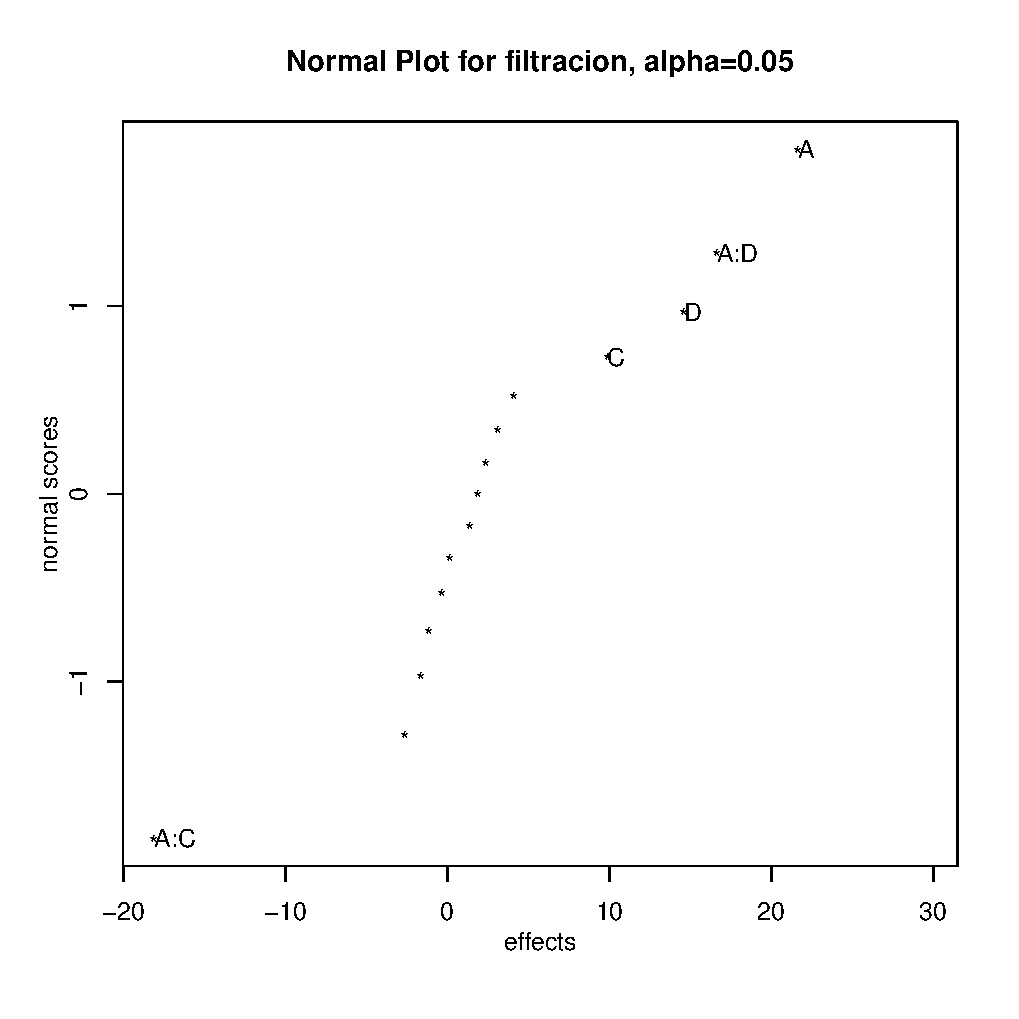
\includegraphics[scale=0.40]{imagenes/DEJ.pdf}
  \caption{Gráfica QQplot de los efectos}
\end{figure}}

\end{frame}

\begin{frame}
\frametitle{Ejemplo de diseño factorial completo con una sola replica}
~\\La ANOVA da como resultado
\begin{table}[H]
  \centering
  \caption{Análisis de varianza una sola réplica}
  \resizebox{0.95\textwidth}{!}{
    \begin{tabular}{cccccc}
    \hline
    \textbf{Fuente de variación} & \textbf{Grados de libertad} & \textbf{Suma de cuadrados} & \textbf{Cuadrados medios} & \textbf{F} & \textbf{$Pr>F$}  \\
    \hline
   \textbf{A} & 1 & 1870.56 & 1870.56& 83.3677& 1.667e-05 ***\\
   \textbf{C} & 1 & 390.06 & 390.06& 17.3844& 0.0031244 **  \\  
   \textbf{D} & 1 &  855.56&  855.56& 38.1309& 0.0002666 *** \\
   \textbf{A:C} & 1 & 1314.06& 1314.06& 58.5655& 6.001e-05 *** \\
   \textbf{A:D} & 1 & 1105.56& 1105.56& 49.2730& 0.0001105 *** \\
   \textbf{C:D} & 1 &   5.06 &   5.06&  0.2256& 0.6474830 \\
   \textbf{A:C:D} & 1 &  10.56 &  10.56&  0.4708& 0.5120321 \\
   \textbf{Residual} & 8 &  179.50 &  22.44 & \\
   
    \hline
    \end{tabular}%
    }
  \label{tab:addlabel}%
\end{table}%       
\end{frame}

\begin{frame}
\frametitle{Ejemplo de diseño factorial completo con una sola replica}
~\\Dado que los únicos efectos significativos son $A=21.625$,$C=9.875$,

$D=14.625$,$AC=-18.125$ y $AD=16.625$, el modelo estimado será
$$\hat{y}=70.06+\left(\frac{21.625}{2}\right)x_1+\left(\frac{9.875}{2}\right)x_3+\left(\frac{14.625}{2}\right)x_4$$
$$-\left(\frac{18.125}{2}\right)x_1x_3+\left(\frac{16.625}{2}\right)x_1x_4$$
\end{frame}


\begin{frame}
\frametitle{Ejemplo diseño fraccionado un medio con una sola replica}

~\\Se retoma el ejemplo anterior y se propone una fracción un medio del diseño $2^4$. Se usará el diseño $2^{4-1}$ con $I=ABCD$. Para construir el diseño, primero se apunta el diseño básico, el cual es un diseño $2^3$. Para encontrar los niveles del cuarto factor, se resuelve $I=ABCD$ para $D$, o $D=ABC$. Por lo tanto, el nivel de D de cada corrida es el producto de los signos positivos y negativos de las columnas A,B y C. El proceso se ilustra en la siguiente tabla
\end{frame}

\begin{frame}
\frametitle{Ejemplo diseño fraccionado un medio con una sola replica}
\begin{table}[htbp]
  \centering
  \caption{Matriz de diseño $2^4$ fraccionado un medio}
  \resizebox{0.85\textwidth}{!}{ 
    \begin{tabular}{ccccccc}
    \hline
    \textbf{Número de} & \multicolumn{3}{c}{\textbf{Diseño básico}} &       & \textbf{Combinación de} & \textbf{Índice de } \\
\cline{2-4}    \multicolumn{1}{p{6.5em}}{\textbf{corrida}} & \textbf{A} & \textbf{B} & \textbf{C} & \textbf{D=ABC} & \textbf{tratamientos} & \textbf{filtración (gal/h)} \\
    \hline
    \textbf{1} & -     & -     & -     & -     & (1)     & 45 \\
    \textbf{2} & +     & -     & -     & +     & ad    & 100 \\
    \textbf{3} & -     & +     & -     & +     & bd    & 45 \\
    \textbf{4} & +     & +     & -     & -     & ab    & 65 \\
    \textbf{5} & -     & -     & +     & +     & cd    & 75 \\
    \textbf{6} & +     & -     & +     & -     & ac    & 60 \\
    \textbf{7} & -     & +     & +     & -     & bc    & 80 \\
    \textbf{8} & +     & +     & +     & +     & abcd  & 96 \\
    \hline
    \end{tabular}%
    }
  \label{tab:addlabel}%
\end{table}%
\end{frame}

\begin{frame}
\frametitle{Ejemplo diseño fraccionado un medio con una sola replica}

~\\Utilizando la relación de definición del diseño $I=ABCD$, podemos deducir que cada uno de los efectos principales es alias de una interacción de tres factores como sigue, $A=BCD$,$B=ACD$,$C=ABD$,$D=ABC$, y además, cada interacción de dos factores es alias de otra interacción de dos factores como sigue, $AB=CD$,$AC=BD$ y $BC=AD$
\end{frame}

\begin{frame}
\frametitle{Ejemplo diseño fraccionado un medio con una sola replica}
~\\En la tabla siguiente se muestran las estimaciones de los efectos obtenidas de este diseño. Para mostrar los cálculos, la combinación lineal de las observaciones asociadas con el efecto de A es
$$L_A=\frac{1}{4}(-45+100-45+65-75+60-80+96)=19 \rightarrow \;\;\; A+BCD $$
~\\Mientras que para el efecto AB se obtendría
$$L_{AB}=\frac{1}{4}(45-100-45+65+75-60-80+96)=-1 \rightarrow \;\;\; AB+CD $$

\end{frame}

\begin{frame}
\frametitle{Ejemplo diseño fraccionado un medio con una sola replica}
\begin{table}[H]
  \centering
  \caption{Estimaciones de los efectos y los alias}
  \resizebox{0.4\textwidth}{!}{
    \begin{tabular}{cc}
    \hline
    \textbf{Estimación} & \textbf{Estructura de los alias} \\
    \hline
  	$L_{A}=19$ & $L_{A} \rightarrow \;\;A+BCD $ \\
  	$L_{B}=1.5$ & $L_{B} \rightarrow \;\;B+ACD $ \\
  	$L_{C}=14$ & $L_{C} \rightarrow \;\;C+ABD $ \\
  	$L_{D}=16.5$ & $L_{D} \rightarrow \;\;D+ABC $ \\
  	$L_{AB}=-1$ & $L_{AB} \rightarrow \;\;AB+CD $ \\
  	$L_{AC}=-18.5$ & $L_{AC} \rightarrow \;\;AC+BD $ \\
  	$L_{AD}=19$ & $L_{AD} \rightarrow \;\;AD+BC $ \\
    \hline
    \end{tabular}%
    }
  \label{tab:addlabel}%
\end{table}% 
\end{frame}

\begin{frame}
\frametitle{Ejemplo diseño fraccionado un medio con una sola replica}
~\\De la tabla anterior, podemos concluir que los efectos principales $A$, $C$ y $D$ son grandes. Además, si $A$, $C$ y $D$ son los efectos principales importantes, entonces es lógico concluir que las dos cadenas de alias de interacciones $AC+BD$ y $AD+BC$ tienen efectos grandes, ya que las interacciones $AC$ y $AD$ también son significativas. Puesto que el factor B no es significativo, puede sacarse de consideración.
\end{frame}

\begin{frame}
\frametitle{Ejemplo diseño fraccionado un medio con una sola replica}
~\\Con base en el análisis anterior, puede obtenerse ahora un modelo para predecir el índice de filtración en la región experimental. Este modelo es
$$\hat{y}=\hat{\beta_0}+\hat{\beta_1}x_1+\hat{\beta_3}x_3+\hat{\beta_4}x_4+\hat{\beta_{13}}x_1x_3+\hat{\beta_{14}}x_1x_4$$
~\\Donde $x_1$,$x_3$ y $x_4$ son variables codificadas $(-1\leq x_i\leq +1)$ y las $\beta$ son los coeficientes de regresión que se obtienen dividiendo la estimación del efecto por 2. Por lo tanto, la ecuación es:
$$\hat{y}=70.75+\left(\frac{19}{2}\right)x_1+\left(\frac{14}{2}\right)x_3+\left(\frac{16.5}{2}\right)x_4+\left(\frac{-18.5}{2}\right)x_1x_3+\left(\frac{19}{2}\right)x_1x_4$$

\end{frame}

\begin{frame}
\frametitle{Conclusión}
~\\La principal conclusión que obtenemos es que los diseños factoriales fraccionados son una alternativa muy útil cuando se tienen muchos factores y los recursos para llevar a cabo el experimento son limitados.

~\\ Observando los dos ejemplos realizados podemos concluir que los diseños factoriales fraccionados son muy importantes, ya que con la mitad o menos de las corridas se llegan a resultados muy semejantes a si se hiciera completo, esto es muy útil ya que en la practica la mayoría de las investigaciones o diseños que se plantean tienen restricciones de recursos y este método es una opción bastante confiable.


\end{frame}



%-----------------------------------------------------------
\begin{frame}
\frametitle{Referencias}
\begin{itemize}

\item Catro, E., Una sola replica del diseño $ 2^{k} $ 
*https://slideplayer.es/slide/6143452/


\item Gromping, U.(2014), 'R package FrF2 for creating and analyzing fractional factorial 2-level designs', Journal
of Statistical Software 56(1), 1-56.
*http://www.jstatsoft.org/v56/i01/


\item Kuehl, R. O. (2001), Diseño de experimentos

\item Salamanca, J. A. C. (2017), 'Análisis factorial múltiple para clasificación de universidades latinoamericanas', Comunicaciones en Estadística .
\end{itemize}
\end{frame}

\begin{frame}
\frametitle{Referencias}
\begin{itemize}

Phoa, F. K., Xu, H. \& Wong, W. K. (2009), "The use of nonregular fractional factorial designs in combination toxicity studies", Food and Chemical Toxicology 47(9), 2183 - 2188. 
*http://www.sciencedirect.com/science/article/pii/S0278691509002701

\item Pulido, H. G. \& de la Vara Salazar, R. (2008), Análisis y diseño de experimentos


\item Wheeler, B. (2014), AlgDesign: Algorithmic Experimental Design. R package version 1.1-7.3. *https://CRAN.R-project.org/package=AlgDesign



\item Villagarcía, T. (n.d.), `Diseños factoriales a dos niveles'
\end{itemize}
\end{frame}

\end{document}